\chapter{Experimenteller Aufbau und Messmethoden}
	\label{chap:exp}

\section{Kryostat und Messaufbau}

Für die im Rahmen dieser Arbeit durchgeführten Experimente wurde ein einfacher Helium"=Badkryostat verwendet. Die Messzelle am unteren Ende des Kryostateneinsatzes kann in das Helium"=Dewargefäß eingebracht werden, wie in Abbildung~\ref{fig:kryostat} zu sehen ist.

\begin{figure}[h!tbp]
	\begin{center}\includegraphics{exp_aufbau/nwa_setup}\end{center}
	\caption[Der verwendete Messaufbau]{Der verwendete Messaufbau. Für Messungen mit Variation des Magnetfelds wurde eine senkrechte supraleitende Magnetspule außerhalb der Messzelle angebracht.}
	\label{fig:kryostat}
\end{figure}

Im Weiteren werden die einzelnen Komponenten des experimentellen Aufbaus genauer beschrieben.

\section{Thermometrie}
Zur Bestimmung der Temperatur des \HR s dient eine geeichte Germanium"=Diode, die direkt am Resonator befestigt ist. Zur Temperaturmessung des Helium"=Bades befindet sich am Boden des Dewargefäßes ein Allen"=Bradley Kohlewiderstand. Desweiteren befindet sich dort auch ein Heizwiderstand, mit dessen Hilfe der Temperaturregler die Temperatur des Heliumbads und somit auch die des darin enthaltenen Experiments regeln und stabilisieren kann. Diese Regelung kann die Temperatur der Messzelle im Bereich von $1.2$ bis \unit[1.8]{K} mit einer Genauigkeit, die kleiner als \unit[0.5]{mK} ist einstellen. Eine weitere, von der beschriebenen Methode unabhängige, Temperaturmessung kann über den in der mit flüssigem $^4$He gefüllten Zelle herrschenden Gasdruck bewerkstelligt werden. Die Temperatur lässt sich über die Dampfdruckkurve von $^4$He bestimmen.
 
\section{Erzeugung von Elektronen}
Bei allen im Rahmen dieser Arbeit durchgeführten Experimente an 2DES werden die Elektronen mittels Glühemission von einem Wolframfilament erzeugt. Die dabei verwendeten Filamente sind Miniaturglühbirnen, deren Glaskörper mit einer Zange angebrochen und entfernt wurden. Bei Raumtemperatur kann man sie bei typischerweise \unit[10]{mA} Strom und \unit[1]{V} Spannung betreiben (d.\,h.\ ihr Widerstand im Betrieb ist ca.\ \unit[100]{$\Omega$} und bei Raumtemperatur ca.\ \unit[20]{$\Omega$}). Bei Temperaturen um \unit[4]{K} sinkt der Kaltwiderstand der Filamente auf bis zu $2$ bis $\unit[3]{\Omega}$ ab.

Um den Wärmeeintrag in das Experiment so gering wie möglich zu halten und auch wegen der besseren Dosierung, werden die Filamente gepulst betrieben. Dabei liegt die Pulslänge im Bereich von $10$ bis $\unit[500]{ms}$ und die Pulsamplitude bei ca.\ \unit[1.2]{V}. Damit das Filament seine Arbeitstemperatur erreicht, muss zu Beginn des Pulses ein starker Strom fließen können. Um den Aufwärmvorgang der Filamente am Beginn des Pulses zu beschleunigen, wurden diese nach \cite{kimitoshi} mit einer niederohmigen\footnote{
Der Leitungswiderstand bei im Experiment üblichen Temperaturen beträgt hier nur einige Ohm.} Zuleitung aus Kupfer angeschlossen. Wenn man eine Konstantspannungsquelle, die zu Beginn des Pulses bis zu \unit[100]{mA} liefern kann, zum Treiben des Filaments verwendet, hat das zur Folge, dass das Filament bereits nach sehr kurzer Zeit seine Betriebstemperatur erreicht (typischerweise $<\unit[10]{ms}$, siehe auch Abb.~\ref{fig:filament_puls}). Zusätzlich gibt es den Vorteil, dass sich das Filament im Betrieb selbst stabilisiert. Da der Widerstand der Zuleitung im Vergleich zum Arbeitswiderstand sehr klein ist, regelt sich an einer konstanten Spannung der Strom durch das Filament so, dass ein Durchbrennen desselben verhindert wird. Wenn das Filament z.\ B. heißer wird, da der Strom durch die Glühwendel zunimmt, steigt sein Widerstand, was wiederum zur Abnahme des fließenden Stromes führt. Der Nachteil des geringfügig höheren Wärmeeintrages durch die Kupferleitung ist im Vergleich zu den dadurch erhaltenen besseren elektrischen Eigenschaften für die Benutzung im Badkryostaten unerheblich.

\subsection{Typische Filamentkennlinien}
\label{ssec:filament}
\begin{figure}[h!tbp]
	\centerline{\hfill\subfigure[Ersatzschaltbild]{\raisebox{0.5cm}{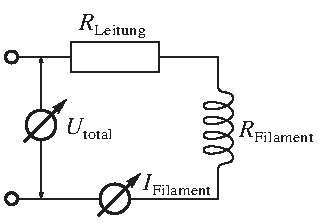
\includegraphics{exp_aufbau/Filamente}}}
	\hfill\subfigure[Verlauf von Strom und Spannung]{\plotlink{filui}{\includegraphics[width=\smallwidth]{exp_aufbau/filui}}}\hfill}
	\caption[Verlauf von Strom und Spannung am Filament]{Schema der Filamentdiagnose und die dabei erhaltenen Daten. In {\bfseries (a)} sieht man das Ersatzschaltbild für den Filamentbetrieb. In {\bfseries (b)} sieht man typische Verläufe von Strom und Spannung während eines Filamentpulses im Experiment.\par(\datalink{2002/mw0201d4/mw0201d4.html}{Messung 01/2002 \#4} Filamentmessung \#100, $U_\text{max}=\unit[1.32]{V}\; I_\text{max}=\unit[104]{mA}$)}
	\label{fig:filamente}
\end{figure}
Zur Kontrolle der Funktion der Filamente wurde der Strom- und Spannungsverlauf während des Pulses aufgezeichnet. Dieser erlaubt so eine genaue Bestimmung der experimentellen Parameter des Filaments.

Aus den in Abb.~\ref{fig:filamente} gezeigten Strom- und Spannungsverläufen eines Filamentpulses kann man über die Bestimmung des Filamentwiderstandes Aussagen über die momentane Temperatur des Filaments machen. Unter der Annahme, dass $R_\text{Leitung}$ während des Pulses konstant und im Bereich einiger Ohm ist, erhält man
\begin{equation}
	\label{eqn:fil_r}
	R_\text{Filament}=\frac{U_\text{total}}{I_\text{Filament}}-R_\text{Leitung}\quad.
\end{equation}

Eine Abschätzung der pro Puls zugeführten Energie kann man aus dem Integral der am Filament aufgewendeten Leistung $P=U\,I$ erhalten, die durch 
\begin{equation}
	\label{eqn:fil_p}
	P_\text{Filament}=U_\text{Filament}I_\text{Filament}=
		\left(U_\text{total}-I_\text{Filament}R_\text{Leitung}\right)I_\text{Filament}
\end{equation}
gegeben ist.
Der vom Strom abhängige Spannungsabfall $U_\text{Leitung}=I_\text{Filament}R_\text{Leitung}$ wird hier zwar noch aufgeführt, später bei der Auswertung der Daten wegen des geringen Leitungswiderstandes jedoch vernachlässigt.

In Abbildung~\ref{fig:filament_puls} sieht man eine Auswertung von Filamentwiderstand und Filamentleistung nach den Gleichungen~\eqref{eqn:fil_r} und \eqref{eqn:fil_p}. Der Filamentwiderstand ist ein Maß für die Temperatur des Filaments und das Integral $E_\text{Fil.}$ über die Filamentleistung ist der Energieeintrag pro Puls in das System, der zum großen Teil verwendet wird, das Filament auf die Arbeitstemperatur aufzuheizen. Die Werte von $R_\text{Fil.}$, $P_\text{Fil.}$ und $E_\text{Fil.}$ sind abhängig vom Gasdruck in der Zelle und auch davon, ob sich das Filament in flüssigem Helium befindet. Alle diese Parameter sind demnach von der Art der Kühlung des Filaments abhängig.

\begin{figure}[h!tbp]
	\centerline{%
	\subfigure[Verlauf des Filamentwiderstands]{\plotlink{filr}{\includegraphics[width=\smallwidth]{exp_aufbau/filr}}}%
	\subfigure[Verlauf der Filamentleistung]{\plotlink{filp}{\includegraphics[width=\smallwidth]{exp_aufbau/filp}}}}
	\caption[Verlauf von Widerstand und deponierter Leistung am Filament]{Der Verlauf {\bfseries (a)} des Filamentwiderstandes und {\bfseries (b)} der im Filament deponierten elektrischen Leistung für die Messdaten aus Abbildung~\ref{fig:filamente} (Aus diesen Daten bestimmte Parameter: $R_\text{max}=\unit[41]{\Omega}$, $R_\text{avg} = \unit[30.4]{\Omega}$, $P_\text{max}=\unit[115]{mW}$, $E=\unit[572]{\grmu J}$). Das Filament erreicht nach ca.\ \unit[10]{ms} seine Endtemperatur. }
	\label{fig:filament_puls}
\end{figure}

\subsection{Durchschnittliche Elektronenproduktion gepulst betriebener Filamente}
\label{ssec:electron_production}

Bei Messungen auf Bulk"=Helium ist durch das Auftreten der elektrohydrodynamischen Instabilität bei $\unit[2\times10^{13}]{\Em}$ ein geeigneter Eichpunkt für die Elektronenproduktion des Filaments vorhanden.
\begin{figure}[t!]
	\centerline{\subfigure[Beladung durch verschiedene Pulsstärken bei $U_\text{clamp}={\unit[100]{V}}$\label{fig:fil_eichung:array}]{\plotlink{fil_eichplot}{\includegraphics{exp_aufbau/fil_eichung}}}}
	\centerline{%
\subfigure[Bestimmung der Instabilität\label{fig:fil_eichung:instab}]{\plotlink{fil_instability}{\includegraphics[width=\smallwidth]{exp_aufbau/fil_instability}}}%
\subfigure[Elektronenproduktion pro Puls\label{fig:fil_eichung:result}]{\plotlink{fil_eichung2}{\includegraphics[width=\smallwidth]{exp_aufbau/fil_eichung2}}}}
	\caption[Eichung der Elektronenproduktion]{Eichung der Elektronenproduktion des Filaments auf Bulk"=Helium. In {\bfseries (a)} ist die Transmission über der Zeit aufgetragen, wobei jeder Datenpunkt einen weiteren Filamentpuls darstellt. Es wurde eine Oberfläche von Bulk"=Helium bei konstanter Haltespannung von \unit[100]{V} und unterschiedlichen Pulsparametern beladen. Aus der anfangs durch die Beladung in {\bfseries (b)} bestimmten Absorption bei Erreichen der elektrodynamischen Instabilität bei \unit[384]{V} kann man die Beladeraten aus den Linienanpassungen von (a) in linearer Näherung abschätzen. In {\bfseries (c)} sieht man die mit dieser Methode bestimmten erhaltenen Elektronenmengen für die Pulse mit unterschiedlichen Parametern. (Messung \datalink{2002/mw0210d1/mw0210d1.html}{mw0210 \#1})}
	\label{fig:fil_eichung}
\end{figure}

Wie in Abbildung~\ref{fig:fil_eichung} zu sehen ist, wurde für eine bestimmte Höhe des Bulk"=Heliums die Spannung ermittelt, bei der die elektrohydrodynamische Instabilität auftritt. Nachfolgend wurden Beladekurven für verschiedene Pulslängen und Pulsamplituden aufgenommen, bei denen eine Spannung an das Substrat angelegt blieb, die geringfügig unter der Spannung bei Instabilität liegt. Dabei kann man in erster Näherung die Transmission als Hinweis auf die Elektronendichte verwenden und die Elektronenproduktion pro Filamentpuls aus der Steigung der abgebildeten Fitgeraden ermitteln.

\subsection{Energieverteilung der emittierten Elektronen}

Die von der Glühwendel emittierten Elektronen besitzen eine gewisse Energieverteilung, die zum einen von ihrer Entstehung durch thermische Emission herrührt und zum anderen durch den linearen Potentialverlauf entlang der Glühwendel bestimmt wird. Die thermische Energie der Elektronen kann man direkt aus ihrer Erzeugung ableiten, wenn man davon ausgeht, dass die thermische Emission bei einer Temperatur von $1500$ bis $\unit[2000]{K}$ stattfindet. Man erhält für diese Temperatur eine korrespondierende thermische Energie von nur ca.\ $\unit[0.2]{eV}$.

Die Energie der emittierten Elektronen, die aus ihrer Beschleunigung durch das elektrische Feld am Filament resultiert, ist einfach abzuschätzen. Da der Betriebswiderstand des Filaments in der Größenordnung von \unit[100]{$\Omega$} liegt und somit viel höher als der Widerstand der Zuleitung ist, fällt fast die gesamte Spannung des Pulses am Filament ab. Wenn man annimmt, dass die Elektronen über die gesamte Länge der Glühwendel emittiert werden, führt dies zu einer Energieverteilung derselben von 0 bis ca.\ \unit[1.2]{eV}.

Die mittlere Stoßzeit von Elektronen in Helium"=Gas bei im Experiment üblichen Temperaturen ist so gering, dass die vom Filament erzeugten Elektronen sehr bald durch Stöße mit den Atomen aus dem Helium"=Gas thermalisieren und daher die Auswirkung ihrer anfänglichen Energie auf den Beladevorgang kaum merkbar ist. Dass die Elektronen sehr gut durch die Stöße mit den Helium"=Atomen im Gasraum abgebremst werden, zeigt sich vor allem bei Messungen mit konstanter, positiver Haltespannung (siehe z.\ B. die Messung der Beladeraten in Abb.~\ref{fig:fil_eichung}). \enlargethispage{\baselineskip}Man findet hierbei kaum Hinweise auf ein verstärktes Durchbrechen der Elektronen.


\section{Bestimmung des Helium"=Füllstands}

\begin{figure}[h!]
	\plotlink{he_level}{\includegraphics[width=\smallwidth]{exp_aufbau/he_level}}
	\hfill
	\begin{minipage}[b]{\textwidth-\smallwidth-\tabcolsep}
		\caption[Abhängigkeit der Resonanzfrequenz vom Helium"=Füllstand]{Beziehung zwischen Resonanzfrequenz und Helium"=Füllstand des mit Substrat bestückten Resonators. Die zwei Knicke in der Mitte bei einem Füllstand von ca.\ \unit[15]{mm} werden durch das Substrat verursacht und können gut als Referenz für das Anpassen der Verschiebung der Resonanzfrequenz an die Höhenskala der Kapazität verwendet werden. Die vertikale Linie bei ca.\ \unit[16]{mm} ist die aus der EHD-Instabilität bestimmte Position der Substrat\-oberfläche. (Messung \datalink{2002/mw0202d3/mw0202d3.html}{02/2002 \#3}, Abschnitt 40)}
		\label{fig:level}
	\end{minipage}
\end{figure}
Zur Bestimmung des Helium"=Füllstands im Resonator kann man die durch das eingefüllte flüssige Helium verursachte Frequenzverschiebung der Resonanz auswerten. Leider ist die Abhängigkeit der Resonanzfrequenz vom Füllstand, wie in Abbildung~\ref{fig:level} zu sehen, nur im Zentrum des Resonators annähernd linear. Man kann zwar unter Vernachlässigung des sich ändernden Resonatorquerschnitts aus dem Frequenzverlauf bei konstanter Abpumprate auf einen linearen Füllstandsverlauf eichen, allerdings gibt es nur einen guten Eichpunkt, der im Frequenzsignal deutlich auszumachen ist -- das Zentrum des Resonators. Wegen der geringen Intensität des elektrischen Feldes der Resonatormoden in der Nähe der Zylinderwand kann man den Start- und Endpunkt des Füllens des Resonators nur sehr schwer festlegen. Hier ist die Frequenzänderung bei Befüllung mit einem Dielektrikum nur sehr gering.

Aufgrund der beschriebenen Schwierigkeit und des Bedürfnisses, den Helium"=Füllstand auch für kleine Füllstände im Resonator für Messungen an Heliumfilmen bestimmen zu können, wurde zusätzlich ein stehender Zylinderkondensator neben dem Resonator in die Zelle eingebaut. Damit lässt sich mit dem flüssigem Helium als Dielektrikum die lineare Abhängigkeit der Kapazität vom Füllstand im Kondensator nutzen, um den Helium"=Füllstand über den kompletten Bereich bis zu einer Genauigkeit von circa $\unit[0.1]{mm}$ zu bestimmen. Die erreichte Genauigkeit ist für die Bestimmung der Filmdicke über den Abstand des Bulk"=Helium"=Füllstandes vom Substrat völlig ausreichend, kann allerdings durch eine genauere Bestimmung der Kapazität noch erhöht werden.

\subsection{Eichung der vertikalen Kondensatorposition}
\label{ssec:level_calib}

Eine Eichung des Helium"=Füllstandes an die vertikale Position des Substrates lässt sich mit Hilfe der elektrohydrodynamischen Instabilität der Elektronen auf Bulk"=Helium durchführen. Bei einer unbekannten Dicke von Bulk"=Helium über dem Substrat bestimmt man durch vorsichtiges Erhöhen der Haltespannung das Einsetzen der elektrohydrodynamischen Instabilität und kann aus der bekannten kritischen Elektronendichte die Dicke des Bulk"=Heliums errechnen. Aus dieser Filmdicke kann man die Position der Substratoberfläche in der aus der Kapazität des Levelkondensators bestimmten Helium"=Füllhöhe bestimmen. Die vertikale Linie in Abb.~\ref{fig:level} soll die so bestimmte Position der Substratoberfläche anzeigen.

\section{Messmethode am Hohlraumresonator}
Üblicherweise liegt die Frequenz von AC-Transportmessungen an 2DES im Bereich
einiger kHz und wird in einer linearen Sommer-Tanner- \cite{Som71} oder einer konzentrischen Corbino"=Elektrodengeometrie realisiert. Wenn man jedoch höhere
Elektronendichten auf dünnen Heliumfilmen erreichen will, ist es schwierig,
eine Transportmessung an den Elektronen mit einem ausreichenden Signal"=Rausch"=Abstand zu realisieren. Denn obwohl das gemessene Signal im Prinzip proportional zu einer Erhöhung der Elektronendichte ist, wird die Substratrauigkeit, die die Beweglichkeit der Elektronen beeinflusst, immer bedeutender. Bei geringen Messfrequenzen ist die durchschnittliche Schwingungsamplitude der Elektronen so groß, dass die Elektronen an der vorhandenen Substratrauigkeit merkbar gestreut werden, was zu einer Reduktion des gemessenen Elektronensignals führt. Abhilfe schafft hier die Verwendung von höheren Frequenzen, um die Transportmessungen bei hohen Elektronendichten auf dünnen Heliumfilmen durchführen zu können. Die Messung der Absorption des 2DES soll bei den zu erreichenden hohen Elektronendichten wegen der auf dünnen Heliumfilmen geringen Mobilität auch bei hohen Messfrequenzen, d.\,h.\ im Mikrowellen"=Frequenzbereich um \unit[10]{GHz} durchgeführt werden. Diese Frequenz ergibt sich aus der Größenordnung der Messanordnung, die im Bereich von Zentimetern liegt. Die Ankopplung an das 2DES geschieht durch die Verwendung von Resonatormoden, deren $\vec E$-Feld parallel zum 2DES liegt.

In Abbildung~\ref{fig:cavity_quer} sieht man einen schematischen Querschnitt durch den verwendeten Hohlraumresonator.
\begin{figure}[h!tbp]
	\centerline{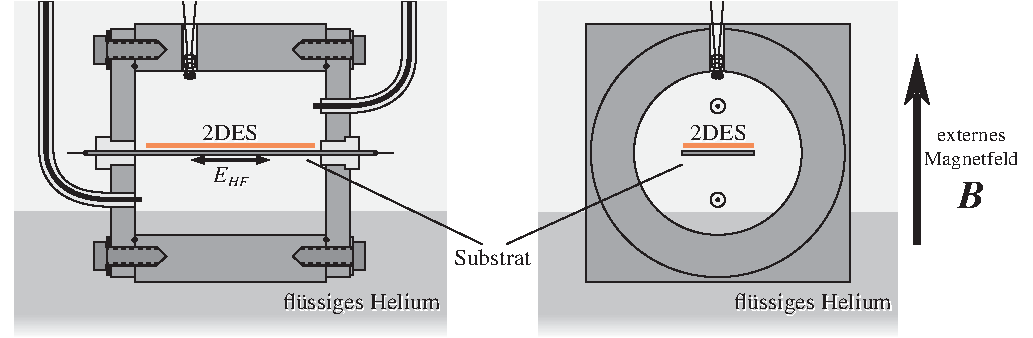
\includegraphics[width=\textwidth]{exp_aufbau/CavityQuerschnitt}}
	\caption[Der Hohlraumresonator im Querschnitt]{Schematische Querschnitte durch den verwendeten Hohlraumresonator. {\bfseries Links} ist ein Querschnitt entlang der Zylinderachse und {\bfseries rechts} ein Querschnitt senkrecht zur Zylinderachse des \HR s zu sehen. Die Länge des Zylinders beträgt \unit[2]{cm} und sein Radius \unit[1.9]{cm}.}
	\label{fig:cavity_quer}
\end{figure}

\subsection{Bisher verwendeter LockIn"=Regelkreis}
\label{ssec:old_method}
\enlargethispage{1\baselineskip}

Der bisher verwendete LockIn-Regelkreis hat den Vorteil, dass das Messsignal sehr schnell Änderungen des Elektronensystems folgen kann. Da die Messfrequenz im Bereich einiger kHz liegt, ist die Antwortzeit der Messung im Bereich von Zehntelsekunden. Dieser Vorteil wird allerdings von dem Nachteil begleitet, dass die Transmission des Resonators nur an einer Frequenz gemessen wird und so die wahre Form der Resonanzlinie verborgen bleibt. Falls die Reflexionen auf den Zuleitungen zum Resonator sehr groß sind oder anderweitig Signalstörungen auftreten, kann man dieses nur schwer diagnostizieren. Das Funktionsprinzip des Regelkreises ist sehr einfach. Der Regelkreis versucht die mittlere Steigung der gemessenen Transmission in einem schmalen Frequenzbereich auf Null zu regeln, d.\,h.\ diese wird genau dann gleich Null, falls die Mittenfrequenz der Frequenzmodulation mit der Resonanzfrequenz des \HR{}s übereinstimmt.

Hierbei wird die Frequenz eines Frequenzgenerators, der im X"=Band\footnote{Dies entspricht einem Frequenzbereich von \unit[8]{GHz} bis \unit[12]{GHz}.} arbeitet, mit Hilfe des Referenzsignals des LockIn-Verstärkers moduliert. Das Signal, das durch den Hohlraumresonator transmittiert, wird über eine Mikrowellendiode mit dem LockIn-Verstärker analysiert und man erhält am Ausgang des LockIn-Verstärkers ein der Steigung der Resonanzkurve am Punkt der Messfrequenz proportionales Regelsignal, dessen Vorzeichen sensitiv auf die jeweilige Flanke der Resonanz des Hohlraumresonators ist. Wenn man das Regelsignal noch in einen PID-Regler einspeist, der daraus einen DC-Offset für das Referenzsignal des LockIn-Verstärkers am Eingang des Frequenzgenerators erzeugt, hat man einen Regelkreis, der sich bei korrekter Justierung immer auf die Frequenz des Maximums der Resonanzlinie einstellt.

Daraus erhält man folgende Parameter der Resonanzfunktion:
\begin{itemize}
	\item Resonanzfrequenz [Hz] und
	\item Amplitude der Transmission an der Resonanzfrequenz [dB].
\end{itemize}
Der Vorteil dieser Methode ist, dass aufgrund der Messfrequenz des LockIn-Verstärkers von einigen Kilohertz das Signal quasi ohne zeitliche Verzögerung messbar ist und somit auch sehr schnelle Änderungen der Resonanz des Hohlraumresonators gemessen werden können, wie sie zum Beispiel nach dem Pulsen des Filaments auftreten. Die Güte der Resonanz wird zu Beginn der Messung abgemessen und im weiteren Verlauf über ihre Proportionalität zur Transmission bestimmt. Im Gegensatz zur in dieser Arbeit verwendeten Messmethode mit dem Netzwerkanalysator wird der \HR\ ständig in Resonanz betrieben, was zur Folge hat, dass der integrale Energieeintrag in das System sehr hoch ist.

\subsection{Neue Messmethode mit Netzwerkanalysator}
\label{ssec:new_method}
Bei Messungen mit Hilfe des Netzwerkanalysators\footnote{Verwendet wurde hier das Modell HP8917D von Hewlett-Packard.} ist die Vorgehensweise eine andere. Mit diesem Gerät ist man in der Lage ein vollständiges Spektrum der Resonanzlinie in der Frequenzumgebung der Resonanz aufzunehmen (typischerweise ist die Frequenzbreite der Abtastung einige MHz,  z.\,B.\ das Doppelte der Linienbreite der Resonanzkurve von ca.\ \unit[10]{MHz}). Für jedes aufzunehmende Spektrum wird die Frequenz der eingestrahlten Mikrowellen kurz über den Messbereich hinweg variiert. Die übliche Zeit für einen Messpunkt, also die Transmission bei einer festen Frequenz ist \unit[0.5]{ms}. Bei typischen 401 Punkten pro aufgenommenem Spektrum ergibt sich eine Gesamtdauer von \unit[200]{ms} pro Spektrum. Nach dieser Messung wird die Mikrowellenemission wieder abgeschalten. Dies ist der größte Unterschied zur bisherigen Messmethode, bei der die Mikrowellen mit genau der Resonanzfrequenz des \HR{}s kontinuierlich in die Zelle eingestrahlt werden, was erhebliche Auswirkungen auf den durchschnittlichen Energieeintrag in das System hat.
	
Die Genauigkeit dieser neuen Messmethode ist allerdings nicht ausreichend, wenn man nur das Resonanzmaximum und dessen Frequenzlage aus den erhaltenen Rohdaten bestimmt. Um eine mit der bisher verwendeten LockIn-Methode vergleichbare Genauigkeit zu erzielen, muss man eine Kurvenanpassung der so erhaltenen Daten der Resonanzlinie an eine einer Lorentzlinie ähnlichen Funktion durchführen:
\begin{equation}
	4A\,\sigma\SQRT{\frac{49x^2 + 4\sigma_\text{res}^2}
	{\left(49\left(x-\nu_\text{res}\right)^2+4\sigma_\text{res}^2\right)
	\,\left(49\left(x+\nu_\text{res}\right)^2+4\sigma_\text{res}^2\right)}}
	+c_0+c_1\nu\quad.
	\label{eqn:resonanzfit}
\end{equation}
\begin{figure}[h!tbp]
	\centerline{%
	\subfigure[Kurvenanpassung der Messdaten]{\plotlink{fitvergleich1}{\includegraphics[width=\smallwidth]{exp_aufbau/fitvergleich1}}}%
	\subfigure[Vergleich der Anpassung mit einem Lorentz-Fit]{\plotlink{fitvergleich2}{\includegraphics[width=\smallwidth]{exp_aufbau/fitvergleich2}}}}%
	\caption[Linienanpassung an die Messdaten der Resonanzkurven]{{\bfseries (a)} Anpassung der Rohdaten nach Gleichung~\eqref{eqn:resonanzfit}. {\bfseries (b)} Vergleich der Linienanpassung nach Gleichung~\eqref{eqn:resonanzfit} mit einem Lorentz"=Fit. (Kurve 1 aus Messung \datalink{2002/mw0205d6/mw0205d6.html}{05/2002 \# 6})}
	\label{fig:fitvergleich}
\end{figure}
Diese Funktion wurde von der Linienanpassung an die Resonanzlinien bei gepulster NMR übernommen \cite{girgl}, die der Autor im Rahmen seiner Diplomarbeit durchgeführt hat. In Abbildung~\ref{fig:fitvergleich} (b) sieht man deutlich das ein Fit mit der einfachen Lorentz-Funktion die Messdaten nicht gut wiedergibt.
Man erhält aus der Kurvenanpassung an Funktion \eqref{eqn:resonanzfit} folgende Parameter:
\begin{itemize}
    \item Resonanzfrequenz $\nu_\text{res}$ [Hz],
    \item Resonanzamplitude $A$ [bel. lineare Einh.],
    \item Linienbreite $\sigma_\text{res}$ [Hz],
    \item konstanter Offset $c_0$ [bel. lineare Einh.] und
    \item linearer Offset $c_1$ [bel. lineare Einh. / Hz].
\end{itemize}
Die beiden Offsetparameter, insbesondere der konstante Offset, sind für die Anpassung realer Messdaten von Nöten. Mit Hilfe des linearen Offsets kann man die Beeinflussung der Messdaten durch nahezu unvermeidbare Leitungsreflexionen erkennen. Diese führen auf Grund der Ausbildung von stehenden Wellen in den Zuleitungen zu einem zusätzlichen von der Frequenz sinusförmig abhängigen Untergrund, dessen Periode groß im Vergleich zur Linienbreite der Resonanzlinie ist und der somit über den Bereich der Resonanz linear genähert werden kann. 

Nach der Linienanpassung wird die daraus bestimmte aktuelle Resonanzfrequenz als Mittenfrequenz des darauffolgenden Frequenzdurchlaufs gesetzt. Somit ist gewährleistet, dass die neue Messmethode mit Hilfe des Netzwerkanalysators immer der Resonanz des Hohlraumresonators folgt -- wie bei der Verwendung des LockIn-Regelkreises.

\begin{figure}[h!tbp]
	\centerline{%
		\subfigure[bisherige Messmethode (LockIn"=Regelkreis)]{\plotlink{vergleich1}{\includegraphics[width=\smallwidth]{exp_aufbau/vergleich1}}}\hfill%
		\subfigure[neue Messmethode (Netzwerkanalysator)]{\plotlink{vergleich2}{\includegraphics[width=\smallwidth]{exp_aufbau/vergleich2}}}}
	\caption[Vergleich der bisherigen und neuen Messmethoden]{Vergleich des bisher verwendeten Regelkreises (siehe Abschnitt~\ref{ssec:old_method}) mit der Netzwerkanalysator"=Methode. Man sieht einen direkten Vergleich einer Beladung mit {\bfseries (a)} der alten und {\bfseries (b)} der neuen Messmethode. Wie man der Abbildung entnehmen kann, ist das Rauschen im Frequenz- und Transmissionssignal bei beiden Messmethoden vergleichbar und in erster Linie von mechanischen Schwingungen des Messaufbaus abhängig. In beiden Fällen wurde ein Beladevorgang durchgeführt, der im Amplitudensignal deutlich zu sehen ist. Vor allem bei Messungen mit Bulk"=Helium in der Zelle wird das Rauschen des Messsignals von den Schwingungen der Heliumoberfläche dominiert. (Messung \datalink{1999/mw9908d1/mw9908d1.html}{08/1999 \#1})}
	\label{fig:alt_neu_vergleich}
\end{figure}

In Abbildung~\ref{fig:alt_neu_vergleich} sieht man einen Vergleich einer Messung des LockIn"=Regelkreises des alten Aufbaus mit der neuen Messmethode mit dem Netzwerkanalysator. Die Rauschamplitude in beiden Messmethoden ist von vergleichbarer Größe und resultiert bei der gezeigten Messung nicht aus dem Rauschen der Messmethode selbst, sondern aus dem Rauschen der Resonanzfrequenz auf Grund von Fluktuationen der Heliumoberfläche im Resonator, die durch Vibrationen des Messaufbaus infolge von Tritt- und Gebäudeschall verursacht werden.

Die Frequenzauflösung beider Messmethoden liegt im Bereich $< \unit[5]{kHz}$ und ist auch für Messungen auf dünnen Heliumfilmen gut geeignet, um dort übliche Frequenzänderungen in der Größenordnung von \unit[100]{kHz} bei Beladung eines dünnen Heliumfilms auf dem Substrat zu detektieren.

Ein Problem, das bei allen Mikrowellenmessungen an 2DES eine Rolle spielt ist, dass die Messung der Parameter der Resonanzlinie synchron zu den Filamentpulsen durchgeführt werden muss. Andernfalls erhält man ein künstliches Rauschen, das das Auftreten der Filamentpulse widerspiegelt.

\section{Zuordnung der verwendeten Moden}
\label{sec:resonatormodes}
\begin{figure}[h!tbp]
	\centerline{%
		\subfigure[Modenstruktur für Variation von $d$]{\plotlink{modeplot1}{\includegraphics[width=\smallwidth]{exp_aufbau/modeplot1}}}%
		\subfigure[Modenstruktur für Variation von $a$]{\plotlink{modeplot2}{\includegraphics[width=\smallwidth]{exp_aufbau/modeplot2}}}%
	}
	\caption[Modenstruktur des \HR s]{Berechnet ist die Modenstruktur nach Gleichung~\eqref{eqn:modenstruktur} in Abhängigkeit von den Parametern des Hohlraumresonators. $d$ ist die Resonatorlänge und $a$ sein Radius. In {\bfseries (a)} ist $a$ auf \unit[0.95]{cm} und in {\bfseries (b)} ist $d$ auf \unit[2]{cm} gesetzt. Die durchgezogene Linie ist der Frequenzverlauf der TM010"=Mode, die zur Messung der Eigenschaften des 2DES verwendet wird. Die gestrichelte Linie zeigt die Frequenz der TM011"=Mode, die auch im betrachteten Frequenzbereich liegt. Für den Parameter $\nicefrac{2a}{d}\approx1$ erhält man auch eine TE111"=Mode in der Nähe der TM010"=Mode, allerdings wird sie aufgrund der Geometrie der kapazitiven Ankopplung an den Seitendeckeln des Resonators nicht angeregt.}
	\label{fig:modeplot}
\end{figure}

Für die in einem zylindrischen Hohlraumresonator angeregten Moden (hier speziell die angeregten TM"=Moden) erhält man in Abhängigkeit von dem Zylinderradius $a$ und der Zylinderhöhe $d$ folgende Beziehung für die Frequenz $\nu$ der jeweiligen Mode:
\begin{equation}
	\label{eqn:modenstruktur}
	\left(2 a \nu\right)=\left(\frac{c k_{ca}(m,n)}{\pi}\right)^2+\left(\frac{c p}{2}\right)^2 \left(\frac{2a}{d}\right)\quad.
\end{equation}

Dies ist eine Geradengleichung für $2 a \nu$ in Abhängigkeit von $\left(\frac{2 a}{d}\right)$; man kann bei einer Auftragung von $2 a \nu$ aus Gleichung~\eqref{eqn:modenstruktur} über $\left(\frac{2 a}{d}\right)$ sehr gut sehen, welche Moden in einem Resonator angeregt werden können.
Für die Werte von $d=\unit[2]{cm}$, $a\approx\unit[0.95]{cm}$ und Frequenzen des leeren Resonators von ungefähr \unit[12]{GHz} kommen die TM010 und die TM011 Moden in Betracht. In Abbildung~\ref{fig:modeplot} sieht man die Frequenz der jeweiligen Moden in Abhängigkeit der Parameter $d$ und $a$. Leider gelten diese Gleichungen nur für den Fall des leeren Resonators. Da die Verschiebung der Frequenz der Moden sowohl von der Dielektrizitätskonstante als auch von Ort und Größe des eingebauten Substrats abhängig ist, kann man die resultierende Frequenzverschiebung für den Fall mit eingebautem Substrat nur abschätzen.

\begin{figure}[h!tbp] 
	\centerline{\includegraphics[width=\textwidth]{exp_aufbau/TM010}}
	\caption[Modenabhängiger Feldverlauf im Resonator der TM010"=Mode]{Der Verlauf der Komponenten des elektrischen Feldes in Zylinderkoordinaten. $E_z$ und $E_r$ der TM010"=Mode sind abgebildet, $E_\phi=0$. Ganz rechts ist der Verlauf von $\abs{\vec E}$ in radialer Richtung dargestellt, der hier unabhängig von der $z$-Koordinate ist. $r$ ist im Bereich [$-a$,\,$a$] und $z$ im Bereich [$0$,\,$d$]. }
	\label{fig:TM010}
\end{figure}

Wie man in Abb.~\ref{fig:TM010} deutlich sieht, ist die TM010"=Mode sensitiv auf Elektronen, die sich auf dem Substrat in der Achse des Resonators befinden. Die TM011"=Mode (siehe Abb.~\ref{fig:TM011}), die ihr maximales elektrisches Feld eher zum Rand des Resonators besitzt, kann als Referenzmode zur Bestimmung des Heliumfüllstands in Randnähe und zur Lokalisierung von Elektronen, die sich nicht auf dem Substrat befinden, verwendet werden.

\begin{figure}[h!tbp]
	\centerline{\includegraphics[width=\textwidth]{exp_aufbau/TM011}}
	\caption[Modenabhängiger Feldverlauf im Resonator der TM011"=Mode]{Der Verlauf der Komponenten des elektrischen Feldes in Zylinderkoordinaten. $E_z$ und $E_r$ der TM011"=Mode sind abgebildet, $E_\phi=0$. Ganz rechts: Verlauf von $\abs{\vec E}$ im Zentrum des Resonators ($z=1$, durchgezogene Linie, erkennbar am Minimum bei $r$=0) und am Rand ($z=0$ oder $z=2$, gestrichelte Linie, ähnlich des Verlaufs bei der TM010"=Mode) in radialer Richtung dargestellt.}
	\label{fig:TM011}
\end{figure}

\subsection{Vergleich des Verhaltens der beiden Resonatormoden}
Wie in Abschnitt~\ref{sec:resonatormodes} gezeigt, kann man mit dem Netzwerkanalysator das Verhalten von zwei unterschiedlichen Resonatormoden quasi gleichzeitig beobachten und so einen Hinweis auf die räumliche Verteilung der Einflüsse des 2DES bekommen.

\begin{figure}[h!tbp]
	\begin{center}
	\subfigure[Transmission]{%
		\plotlink{modevgl_bulkt}{\includegraphics[width=\ssmallwidth]{exp_aufbau/modevgl_bulkt}}}%
	\subfigure[Resonanzfrequenz]{%
		\plotlink{modevgl_bulkf}{\includegraphics[width=\ssmallwidth]{exp_aufbau/modevgl_bulkf}}}
	\end{center}
	\caption[Gemessenes Verhalten beider Resonatormoden mit 2DES im Resonator]{Vergleich der beiden erreichbaren Resonatormoden TM010 und TM011 bei einer Beladung von Bulk"=Helium. Es ist deutlich zu sehen, dass die TM011"=Mode weniger sensitiv auf das Elektronensystem ist, das sich hauptsächlich im Zentrum des \HR s befindet.\par ($T_0(\text{TM010})=\unit[34.1]{dB}$, $T_0(\text{TM011})=\unit[43.2]{dB}$, $\nu_0(\text{TM010})=\unit[9.5847]{GHz}$, $\nu_0(\text{TM011})=\unit[11.929]{GHz}$; Messung \datalink{2000/mw0008d2/mw0008d2.html}{08/2000 \#2}, Messpunkt 1055--1087)}
	\label{fig:tworesonance}
\end{figure}

In Abbildung~\ref{fig:tworesonance} sieht man das Verhalten von Transmission und Resonanzfrequenz für die TM010 und die TM011"=Mode während einer Beladung von Bulk"=Helium. Da sich bei der TM010"=Mode, wie in Abbildung~\ref{fig:TM010} zu sehen, das Maximum der Feldverteilung entlang der Symmetrieachse des Resonators befindet und dies auch der Ort ist, an dem sich das Substratplättchen mit den Elektronen auf der Heliumschicht befindet, ist der Einfluss auf die Änderung der Modenparameter deutlich stärker als bei der TM011"=Mode. Für die TM011"=Mode befindet sich der Ort der maximalen Feldamplitude zwischen Zentrum und Rand des Resonators, also in einem Bereich, in dem sich durch die zentrale Lage des Substratplättchens bedingt weniger Elektronen befinden. Deshalb zeigt das allgemeine Verhalten der TM011"=Mode im Vergleich zur TM010"=Mode bei Beladung des Substrats mit Elektronen einen schwächeren Einfluss. Die Änderung des Verhältnisses von TM010"= und TM011"=Mode während einer Messung kann wichtige Hinweise auf die Verteilung von Elektronen im Resonator liefern (siehe Abschnitt~\ref{ssec:pmma_reproduce} auf Seite~\pageref{ssec:pmma_reproduce}).

\section{Vergleich der gemessenen Transmissions- und Gütewerte}
\label{sec:transquality}
Da die Messmethode mit dem Netzwerkanalysator erstmals die Möglichkeit bietet, die Resonanzparameter Transmission und Güte gleichzeitig und unabhängig voneinander zu bestimmen, soll das Verhalten dieser Werte hier für eine typische Messung betrachtet werden.

Die Absorption $\nicefrac1{Q_e}$ des Elektronensystems ergibt sich aus der Resonatorgüte ohne 2DES ($Q_0$) und mit 2DES ($Q_\text{beladen}$) nach folgender Gleichung:
\begin{equation}
	\label{eqn:absorption}
	\frac1{Q_e}=\frac1{Q_\text{beladen}}-\frac1{Q_0}\quad.
\end{equation}
In der Dissertation von \name{Günzler} \cite{guenzler} wurde für die Berechnung der Absorption aus der gemessenen transmittierten Leistung $P$ folgende Gleichung verwendet, wobei im Falle des Netzwerkanalysators die Transmission $T$ direkt gemessen wird:
\begin{equation}
	\label{eqn:absorption_trans}
		\frac1{Q_e}=\frac1{Q_0}\left(\sqrt{\frac{P_0}{P}}-1\right)=
			\frac1{Q_0}\left(\frac{T_0}{T}-1\right)\quad.
\end{equation}

\begin{figure}[h!tbp]
	\centerline{%
	\subfigure[auf \SiO\ (\datalink{2002/mw0202d2/mw0202d2.html}{02/2002 \# 2}, Abschnitt 20)]{\plotlink{absorp1}{\includegraphics[width=\smallwidth]{exp_aufbau/absorp1}}}%
	\subfigure[auf PMMA (\datalink{2002/mw0204d4/mw0204d4.html}{04/2002 \# 4}, Abschnitt 84)]{\plotlink{absorp2}{\includegraphics[width=\smallwidth]{exp_aufbau/absorp2}}}}%
	\caption[Vergleich der Berechnung der Absorption aus Tranmission oder Güte]{In {\bfseries (a)} sieht man einen Vergleich der Absorptionswerte, die zum einen aus der gemessenen Güte nach \eqref{eqn:absorption} und zum anderen aus der gemessenen Transmission nach \eqref{eqn:absorption_trans} berechnet wurden. Im eingesetzen Graph sieht man, dass der Quotient aus den berechneten Absorptionswerten mit zunehmender Elektronendichte größer wird. Im Falle einer Beladung von PMMA"=Substrat {\bfseries (b)} mit um einen Faktor 10 geringerem Absorptionswert stimmen die unabhängig voneinander berechneten Absorptionswerte gut überein.}
	\label{fig:absorption}
\end{figure}

\enlargethispage{\baselineskip}
In Abbildung~\ref{fig:absorption} sieht man die nach Gleichung \eqref{eqn:absorption} und \eqref{eqn:absorption_trans} berechneten Absorptionswerte. Bei den hohen Elektronendichten in Teilabbildung {\bfseries (a)} sieht man auch eine Abweichung von der bisherigen Annahme, dass die gemessene Transmission proportional zur Güte des Resonators ist. Bei geringen Elektronendichten wie z.\ B. in Teilabbildung {\bfseries(b)}  ist die Bestimmung der Absorption aus der Transmission äquivalent zu ihrer Bestimmung aus der Güte.


